\documentclass[a4,center,fleqn]{NAR}

% Enter dates of publication
\copyrightyear{2020}
\pubdate{31 December 2020}
\pubyear{2020}
\jvolume{XX}
\jissue{YY}

%\articlesubtype{This is the article type (optional)}

\begin{document}

\title{Mapping short reads, faithfully}

\author{%
Eduard Valera Zorita\,$^1$,
Ruggero Cortini\,$^1$,
Guillaume J. Filion\,$^{1,2,3}$
\footnote{To whom correspondence should be addressed.
Email: guillaume.filion@gmail.com}}

\address{%
$^{1}$Center for Genomic Regulation (CRG), The Barcelona Institute
of Science and Technology, Dr. Aiguader 88, Barcelona 08003, Spain;
$^{2}$University Pompeu Fabra (UPF), Barcelona, Spain;
$^{3}$present address: Department of Biological Sciences, University
of Toronto Scarborough, Toronto, ON, Canada.}
% Affiliation must include:
% Department name, institution name, full road and district address,
% state, Zip or postal code, country

\history{%
Received January 1, 2009;
Revised February 1, 2009;
Accepted March 1, 2009}

\maketitle

\begin{abstract}
Mapping is the process of finding the original location of a DNA read in a
reference sequence, typically a genome. Short read mappers are used in
most applications of high-throughput sequencing. As such, they must be
continuously improved to keep up with increasing needs. To gain speed,
many mappers rely on seeding heuristics that can negatively affect the
mapping accuracy. For lack of a method to compute such probabilities,
mappers have so far used \textit{ad hoc} approximations of variable
quality. Here we devise the elements of a strategy to map short reads
faithfully, \textit{i.e.}, to provide accurate probabilities of mapping
errors. The key is to estimate the number of paralogus of the target so as
to spend more time on the reads that can be mapped with high confidence.
This strategy highlights the existence of a class of reads that can be
mapped with unprecedented confidence. We implement this strategy in a
prototype mapper that is competitive with state-of-the-art mappers BWA-MEM
and Bowtie2, with the benefit of faithfulness. The software is open-source
and availble from \url{https://github.com/gui11aume/smmfdp}.
\end{abstract}


\section{Introduction}

High throughput DNA sequencing is now a well-established technology with
countless applications in industry and medicine~\cite{pmid30084865}. The
Illumina short-read technology currently dominates the market of DNA
sequencing, so the software exploiting this technology is an important
target for optimization~\cite{Wikillu}.

After sequencing, reads are usually mapped to a known reference, typically
a genome, using a software tool known as a mapper. The main challenge is
that sequencers sometimes make mistakes, so mappers must solve an
approximate string-matching problem. The traditional vision of mapping
algorithms is to optimize speed and accuracy while maintaining a low
memory footprint. From this perspective, a major breakthrough was the
conception of the FM-index~\cite{ferragina2000opportunistic,
ferragina2005indexing}, a data structure based on the Burrows-Wheeler
transform~\cite{burrows1994block} and on the suffix
array~\cite{manber1993suffix}. Modern short-read mappers such as
BWA-MEM~\cite{li2013aligning} and Bowtie2~\cite{pmid22388286} rely on
specialized implementations of the FM-index for DNA sequences. More
recently, new mapping algorithms for specific applications such as RNA-seq
have further improved the speed and the accuracy in some
areas~\cite{pmid27043002}.

However, speed, accuracy and memory usage are not the only metrics that
matter for mapping algorithms. Equally important is an attribute called
\emph{faithfulness}.

Faithfulness comes into play for heuristic algorithms, \textit{i.e.},
algorithms that may return an incorrect result. We say that a heuristic is
\emph{faithful} if it provides an accurate probability that the result is
incorrect. Importantly, faithfulness is orthogonal to accuracy in the
sense that a faithful algorithm is not necessarily accurate and
\textit{vice versa}.

% **************************************************************
% Keep this command to avoid text of first page running into the
% first page footnotes
\enlargethispage{-65.1pt}
% **************************************************************

The importance of faithfulness is recognized in the specifications of the
SAM format \cite{pmid19505943}, featuring a mandatory \emph{mapping
quality} field MAPQ, defined as ``$-10 \cdot \log_{10}Pr$\{mapping
position is wrong\}''. However, the proposed methods to estimate this
probability are accurate only for some genomes and some sequencing
technologies.
THIS NEEDS TO BE WRITTEN BETTER.
%However, there is presently no way to estimate this
%probability, and therefore no way to respect the standard.
Some mappers
like STAR~\cite{pmid23104886} use the MAPQ field as a qualitative scale.
%Some others like GEM~\cite{pmid23103880} do not provide a mapping quality.
As for the mappers aiming to comply with the SAM standard, the scores are
undocumented, variable between mappers and versions, often spreading
puzzlement and frustration in the community~\cite{ACGT, QCFail}.

As a consequence, mapping quality is often neglected by users and
developpers, even though it is critical in many applications. For
instance, when calling \textit{de novo} mutations, the standard procedure
is to map sequencing reads to the genome of interest, and score mismatches
as evidence for mutations. Mapping errors can also explain the mismatches,
so the confidence in the final call is commensurate with the mapping
quality. Inaccuracies of the MAPQ estimates cause recurrent errors in
cancer genomics~\cite{dunno} where faithfulness would make a major
difference.

Mapping quality is also important in multi-genome or multi-reference
applications. For instance, in experiments on chimeras, the confidence
that a read is mapped to the correct location is in fact the confidence
that the read is assigned to the correct genome. Applied to RNA-seq,
mapping quality thus dictates mono-allelic expression calls; applied to
Hi-C it dictates the inferred contact map of the chromosome. More
generally, in this context every analysis depends on the confidence in
the locations of the reads.

Improving the mapping process requires to understand why it is sometimes
inaccurate in the first place. Mapping heuristics are usually based on a
filtration strategy called \emph{seeding}, whereby short matches between
the read and the reference are used to extract a set of candidate
locations. Seeding is error-prone because the correct location of the read
may be filtered out. We recently developped a formal computational
framework to compute the error rate of different seeding strategies used
for mapping short reads~\cite{Filion619155}. Missing from this framework
was a method to estimate the unknown parameters of the model.

Here we propose a method to estimate those parameters and we implement it
in a mapper called MEM Mapper Prototype (MMP) that aims to be faithful. We
use MMP to study the feasibility of this strategy and we highlight the
additional benefits gained from faithfulness. In the process, we discover
a class of reads that can be mapped with extremely high confidence and we
show that faithfulness can be achieved without sacrificing speed or
accuracy.


\section{MATERIALS AND METHODS}

\subsection{Estimating $N$ from the backward search}

We assume that the true location of the read is a sequence of the genome
that has $N \geq 0$ duplicates. For every nucleotide, the probability that
a duplicate differs from the target is a constant $\mu$, and the
probability that the read differs from the target is a constant $p$. We
further assume that the genome has size $G$ and that its composition is a
equiprobable random mix of the four nucleotides.

For every nucleotide, the probability that the read differs from a given
duplicate is $\lambda = (1-p)\mu + p(1-\mu/3)$. The probability that the
duplicate matches the last $L$ nucleotides of the read is thus $a_L =
(1-\lambda)^L$, and the probability that at least one of the the $N$
duplicates matches them is $1-(1-a_L)^N$. Finally, the probability that
some duplicate matches the last $L$ nucleotides of the read, but none
matches the last $L+1$ is $\ell(L|N) = (1-a_{L+1})^N-(1-a_L)^N.$

From the expression above, it is possible to estimate $N$ by the maximum
likelihood method. For this, we need to find the value of $N$ that
maximizes $\ell(L|N)$ for fixed $L$. This can be done analytically by
solving $\partial \ell / \partial N = 0$, yielding
\begin{align}
\label{eq_mle}
\hat{N}(L) =\frac{ \log \big( \log(1-a_{L+1}) / \log(1-a_L) \big)} {
\log(1-a_{L+1}) - \log(1-a_L) }.
\end{align}

In practice, we can compute $L$ with the backward search by extending the
query until there are fewer than two hits in the genome (when there is
only one hit, it is most likely the target). This is not exactly a maximum
likelihood estimate because we should specifically account for the target
as one of the hits. Also, $\mu$ is usually unknown, so we take a
conservative approach and set $\mu$ to a value where the recall is low for
reads in the range 50--150~bp (for MEM seeds we set $\mu = 0.06$).

Finally, the formula is symmetric so we can obtain two estimates of $N$,
one from each end of the read, and average them for more robustness. Note
that expression (\ref{eq_mle}) is a maximum likelihood estimate, but the
final estimate of $N$ is not, because of the approximations mentioned
above.

\subsection{Computing MAPQ}

\subsubsection{Super quality} Super reads are defined as reads that
satisfy the two following conditions: 20-mers extracted every 10
nucleotides all have a single hit in the genome (see the Results section
and Figure~\ref{fig_supertest}), and the read is mapped without mismatch.

Super reads are mapped to an incorrect location if $i.$ the target has
exactly one duplicate, $ii.$ the read contains $m$ errors, $iii.$ the
paralog differs from the target exactly at the $m$ locations of the
errors, $iv.$ the $m$ incorrect nucleotides match the paralog, and $v.$
the $m$ errors are in the odd-numbered 10-mers of the read. The
justification for these conditions are explained in more detail in
Figure~\ref{fig_supread}.

Condition $v.$ imposes $m = 1 + \lfloor L/20 \rfloor$ for a read of size
$L$. The probability of $i.$ is denoted $\alpha$. The probability of $ii.$
is ${L \choose m}p^m(1-p)^{L-m}$, where $p$ is the error rate of the
sequencer. The probability of $iii.$ is $\mu^m(1-\mu)^{L-m}$, where $\mu$
is the probability that the duplicate differs from the target. The
probability of $iv.$ is $1/3^m$. The probability of $v.$ is $10^m/{L
\choose m}$. We need to multiply those terms together and divide them by
the probability that a read is super, which is fraction $\beta$ of the
probability that a read has no error. The mapping quality of super reads
is finally computed as
\begin{align}
\label{eq_super}
\frac{\alpha}{\beta} \left( \frac{3.33 \cdot p\mu}{1-p}
\right)^m (1-u)^{L-m}.
\end{align}

The parameter $\mu$ is set to $m/L$ so as to maximize (\ref{eq_super}),
and $\alpha/\beta$ was observed empirically to be close to 0.1.


\subsubsection{Normal quality} Reads with initial estimate $N \leq 20$ are
mapped by checking all the candidates. The prior probability that the true
location is not discovered can be calculated with
\texttt{sesame}~\cite{Filion619155}. We can gain precision by computing the
posterior probability given the number of mismatches (intuitively, a large
number of mismatches is evidence that the read is mapped to an incorrect
location). If the read is mapped to the correct location, the number of
errors follows a binomial distribution where the parameter $p$ is the
error rate of the sequencer. If it is mapped to a paralog, the parameter
is $\lambda$ as defined above. A complication is that the distribution of
errors is not binomial when $N > 1$ because the best hit is not chosen
randomly among the $N$ paralogs. We thus compute the posterior probablity
using Bayes formula, but put an upper threshold equal to 1 on the
log-ratio of the evidence. This means that many mismatches is strong
support for an incorrect location, but few mismatches is only weak support
for the correct location.

Assuming that the read is mapped with $x$ mismatches, the probability that
the location is incorrect is computed as
\begin{align}
\label{eq_bayes}
P(N \geq 1) \cdot \frac{P_s}{P_s + (1-P_s)e^{\min(a-b,1)}},
\end{align}
where $P_s$ is the prior probability provided by \texttt{sesame}, where
$a-b=x \cdot \log(p/\lambda)+(L-x) \cdot \log((1-p)/(1-\lambda))$, and
where $P(N \geq 1)$ is a probability computed during the estimation of $N$
(see below).

It was verified empirically, that expression (\ref{eq_bayes}) is an
overestimate when $x = 0$. In this case, the estimate is replaced by a
direct approach where we compute the probability that a paralog matches
the read perfectly. More specifically, we compute the probability that the
read has exactly one error and that a paralog matches the incorrect
sequence. In this case, the probability that the location is incorrect is
computed as
\begin{align}
\label{eq_x0}
P(N \geq 1) \cdot \frac{Lp(1-p)^{L-1}
\left(1-\left((1-\mu)^{L-1}\mu/3\right)^N\right)}{(1-p)^L}.
\end{align}

In both (\ref{eq_bayes}) and (\ref{eq_x0}), $\mu$ is set to 0.06 as this
gives a high proability that MEM seeding fails for reads of size 50--150.


\subsubsection{Low quality} Reads with initial estimate $N > 20$ are
mapped by checking only the longest MEM seed. A seed of size $S$ exists if
there are $S$ nucleotides without error or if there are $S$ nucleotides
with an error matching at least one of the $N$ paralogs. In the first
case, the target is discovered, in the second it is not. We also have to
count whether seed is limited by errors or by the end of the read.
The probability of the first case is
\begin{align*}
P_{\text{hit}} = \delta_L \cdot (1-p)^S \cdot \delta_R,
\end{align*}
where $\delta_{L/R} = 1$ if the seed is flanked by the end of the read and
$p$ otherwise.

Counting only the most frequent case with a single error, the probability
of the second case is
\begin{equation*}
\begin{split}
P_{\text{miss}} = \; &\delta_L \cdot Sp(1-p)^{S-1} \cdot \delta_R  \\
   &\times \left(1- \left( 1-\delta_L' \cdot(1-\lambda)^{S-1}\lambda/3
   \cdot \delta_R'\right)^N \right),
\end{split}
\end{equation*}
where $\lambda$ is defined as above, and where $\delta_{L/R}' = 1$ if the
seed is flanked by the end of the read and $\lambda$ otherwise. Applying
Bayes' formula, the mapping quality is finally computed as

\begin{align}
\label{eq_low}
\frac{P_{\text{miss}}}{P_{\text{hit}} + P_{\text{miss}}}.
\end{align}

\subsubsection{Estimating $P(N \geq 1)$.} This quantity appears in
expressions (\ref{eq_bayes}) and (\ref{eq_x0}). The estimate is based on
the method shown in Figure~\ref{fig_back}, where we use the end of the
read with the shortest query. We consider three cases: $i.$ the target has
a paralog, $ii.$ only one end of the target has a paralog, and $iii.$ the
target is unique. Case $ii.$ can occur when the read straddles the end of
a transposon or other repeated sequence. We consider that $N \geq 1$ only
in case $i.$ where the sequence has a full-length paralog.

We denote $m$ the longest query size with two more more hits in the genome
(see Figure~\ref{fig_back}) and we write $P(m)$ in the three cases above.
The genome has size $G$ and every nucleotide matches the query with
probability $1/4$ if it is unrelated to the target, and with probability
$\lambda$ if it is a paralog. For convenience, we also define the
probability of a random hit of size less than $m$ as $\xi(m) = 1-1/4^m$.

In case $i.$, the observed value is $m$ if there is a match of size $m$
with the paralog at one end of the read, and a match of size $\geq m$ at
the other end, and a match of size $< m$ with the rest of the genome;
or if the match with the paralog has length $< m$ at both ends of the
read, and there is a match of size $m$ with the rest of the genome; or if
there is a match of size $m$ with the paralog at one end of the read, and
a match of size $\geq m$ at the other end, and a match of size $m$ with
the rest of the genome. In case $i.$, $P(m)$ is thus
\begin{align*}
P_1 = \lambda (1-\lambda)^{2m} \xi(m)^G + \\
\big(1-(1-\lambda)^m\big)(1-\lambda)^m \big(\xi(m+1)^G - \xi(m)^G\big) + \\
\lambda (1-\lambda)^{2m} \big(\xi(m+1)^G - \xi(m)^G\big).
\end{align*}

In case $ii.$, the observed value is $m$ if there is a match of size $\geq
m$ with the paralog at the duplicated end, and a match of size $m$ with
the rest of the genome at the other end; or if there is a match of size $<
m$ with the paralog at the duplicated end, and a match of size $m$ with
the rest of the genome at any end, and a match of size $\geq m$ at the
other end. In case $ii.$, $P(m)$ is thus
\begin{align*}
P_2 = (1-\lambda)^m \big((\xi(m+1)^G - \xi(m)^G\big) + \\
\big(1-(1-\lambda)^m\big) \big(\xi(m+1)^G - \xi(m)^G\big)
\big(1 - \xi(m)^G\big).
\end{align*}

In case $iii.$, the observed value is $m$ if there is a random match of
size $m$ with the genome at one end of the read, and a random match of
size $\geq m$ at the other end. In case $iii.$, $P(m)$ is thus
\begin{align*}
P_3 = \big(1-\xi(m+1)^G\big) \big(\xi(m+1)^G - \xi(m)^G\big).
\end{align*}

Finally, to compute the probability of case $i.$ given the observed value
of $m$, we use Bayes formula with prior odds in proportion $1:1:8$ because
we estimate that the probability that a sequence has exactly one paralog
is approximately $1/10$ (remember that those calculations are performed
when there is evidence that $N \leq 20$).

\begin{align*}
P(N \geq 1) = \frac{P_1}{P_1 + P_2 + 8\cdot P_3}.
\end{align*}


\subsection{MMP implementation}

MMP is implemented as a stand-alone C program including the code of
\texttt{sesame}~\cite{Filion619155} and of
\texttt{divsufsort}~\cite{fischer2017dismantling}. MMP uses a standard
implementation of the FM-index for the genome and its reverse complement,
as detailed in~\cite{blog}, and of the Needleman-Wunsch
algorithm~\cite{pmid5420325}, with the modification that the algorithm is
interrupted if the score rises above that of the current best hit. During
indexing, the backward search~\cite{ferragina2000opportunistic} is carried
out on all possible 12-mers and the results are stored so that the first
12 iterations of every query can be skipped during the mapping.

The implementation otherwise follows the flow chart of
Figure~\ref{fig_tree} using the formula above, with two differences.
The first is that super reads can have 0, 1 or two mismatches, as long as
all the extracted 20-mers have a single hit in the genome. How mapping
quality is computed in those cases is described in the Supplementary
Material. The second difference is that once the best hit is found, $N$ is
estimated again on the genome instead of the read, and the higher of the
two estimates is kept.

\subsection{Benchmark}

\subsubsection{Genomes and data sets}

The main characteristic of the genomes used for benchmark
(\textit{Drosophila melanogaster}, \textit{Homo sapiens} and \textit{Pinus
taeda}) are summarized in Table~\ref{table_genomes}.

\begin{table}[b]
\tableparts{%
\caption{Features of the genomes used for benchmark.}
\label{table_genomes}%
}{%
\begin{tabular*}{\columnwidth}{@{}llrr}
\toprule
Organism & Reference & Size & Sequences \\
\colrule
\textit{Drosophila melanogaster} & dm4/R6 & 150~Mbp & 1,870 \\
\textit{Homo sapiens} & hg38/GRCh38 & 3.27~Gbp & 455 \\
\textit{Pinus taeda} & GCA\_000404065.3 & 22.50~Gbp & 1,760,464 \\
\botrule
\end{tabular*}%
}
{}
\end{table}

The data sets used for benchmark consist of 50 million sequences drawn
uniformly at random from each genome. To simulate sequencing errors,
nucleotides were randomly substituted with a fixed probability; there were
no insertions or deletions. For each data set, the sequences have the same
length (50, 75 or 100 nucleotides) and the same error rate (1\%, 2\%, 5\%
or 10\%).

\subsubsection{Software}

We used BWA-MEM version 0.7.9a-r786~\cite{li2013aligning}, Bowtie 2
version 2.3.5.1~\cite{pmid22388286}, and MMP version 1.0. The genomes were
indexed with default parameters for each mapper. For the benchmark proper,
all the mappers were run in single thread. BWA-MEM and Bowtie2 were always
used with default options, and the \texttt{-e} flag of MMP was used to
specify the error rate of the data set, \textit{e.g.}, \texttt{-e .02} for
a 2\% error rate.

\subsubsection{Hardware}

All the mapping experiments were run on a Hewlett Packard Z800 workstation
with 64~bit Intel Xeon CPU X5675 at 3.07~GHz, with 64~GB of DDR3 RAM,
12~MB of cache, and running Linux Ubuntu 18.04.3. Indexing the pine genome
with MMP had to be done on a machine with 512~GB of RAM because of the
high memory footprint used by the library \texttt{divsufsort}.


\section{RESULTS}

\subsection{General design principle of a faithful mapper}

Implementing a faithful mapper requires a theory to estimate the
probability that the location of a read is wrong. We recently showed that
most of the errors can be attributed to the seeding step and we developed
a computational framework to estimate the error rate of different seeding
schemes~\cite{Filion619155}. If we want those probabilities to correspond
to the overall error rate of the mapper, it is important to verify all the
candidate locations after the seeding step, otherwise neglecting some
candidates would introduce some further mapping errors with unknown
probability.

We thus opted to implement a mapper based on MEM seeds (where MEM stands
for Maximal Exact Match) because this strategy produces a smaller
candidate set than the alternatives. In order to optimize the design of
the filtration step, we used the \texttt{sesame}
library~\cite{Filion619155} to sketch the projected performance of MEM
seeds (Figure~\ref{fig_MEM}).

\begin{figure}[t]
\begin{center}
\includegraphics[scale=.6]{MEM_19.pdf}
\end{center}
\caption{Projected performance of MEM seeds. The probability that the
target is not in the candidate set after seeding  is plotted against the
size of the read (notice the log scale on the $y$ axis). Computations are
carried out with \texttt{sesame} for MEM seeds of minimum size 19,
assuming an error rate of 1\% and a divergence rate of 6\% between
paralogs (the probability that a given nucleotide of the target is
different in a given paralog is 0.06). Each line represents the
probabilities for a different number $N$ of paralogs. Note that the
asymptotic decay is approximately constant up to $N = 20$ and slows down
for larger $N$.}
\label{fig_MEM}
\end{figure}

The results reveal two essential insights: The first is that the
asymptotic decay of the failure rate is approximately constant when the
read maps to a location with 20 or fewer duplicates. Beyond this, the
asymptotic decay slows down and the recall decreases markedly. The second
insight is that up to 100 nucleotides, the failure rate is always above 1
error per 100,000 reads. In other words, there is no hope to map a read
with high confidence using MEM seeds if the target has a paralog.

These insights suggest that an efficient strategy is to use a fast mapping
mode when the target has many duplicates because the read cannot be mapped
with high confidence anyway. In contrast, when the number of duplicates is
low, it is important to know whether the target is a unique sequence
because this is the only way to map a read with high confidence. So after
MEM seeding, our strategy is to quickly estimate the number of duplicates,
find a decent candidate location as fast as possible and finally estimate
how reliable this location is. In other words, we search the reads that
can be mapped with high confidence instead of searching a high-confidence
location for every read. A high-level summary of this strategy is shown in
Figure~\ref{fig_tree}.

\begin{figure}[t]
\begin{center}
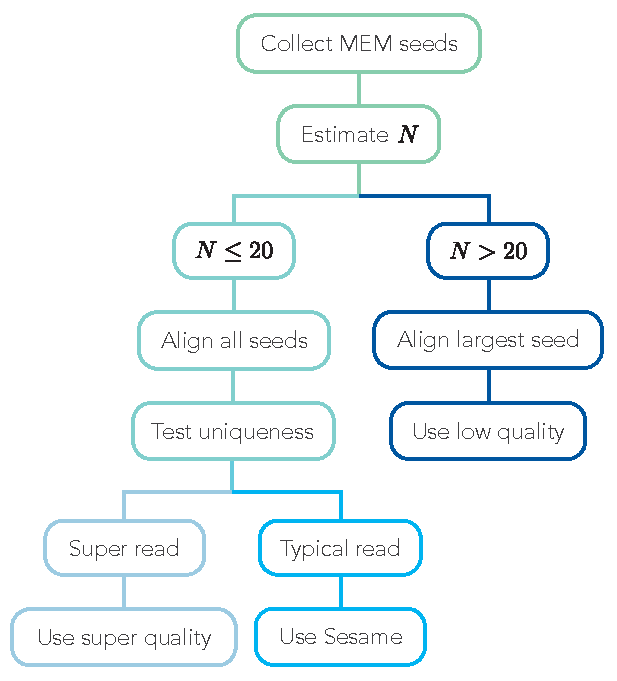
\includegraphics[scale=.8]{decision_tree.pdf}
\end{center}
\caption{Proposed strategy for a faithful mapper. Each read is routed
through a different mapping pathway. First, all the MEM seeds are
extracted (top). Then the number $N$ of paralogs of the target is
estimated. If $N$ is 20 or less (left branch), all the candidates are
tested with the Needleman-Wunsch algorithm. Once the best candidate is
found, the probability that it is unique is estimated. If it is high and
the alignment has no mismatch, mapping quality is computed using
(\ref{eq_super}). If the best candidate is not unique or if the alignment
has a mismatch, mapping quality is computed using (\ref{eq_bayes}) or
(\ref{eq_x0}). If $N$ is higher than 20 (right branch), only the largest
MEM seed is used and the mapping quality is computed using (\ref{eq_low}).
}
\label{fig_tree}
\end{figure}


\subsection{Estimating $N$}
\label{sec_N}

The key in the flow chart of Figure~\ref{fig_tree} is to dispatch the
reads based the number $N$ of paralogs of the target, which is an
indirect measure of the mappability of the read~\cite{pmid22276185}.
Estimating $N$ must be fast so that this step does not become a
bottleneck. To achieve this, we propose to use the seeding process itself.
MEM seeds are best computed using the backward
search~\cite{ferragina2000opportunistic}, an algorithm that returns the
number of hits in the genome as the query is extended backward. If the
target has no or few paralogs (Figure~\ref{fig_back}a), the number of hits
will quickly go below 2 (when there is only one hit, it is most likely the
target itself). In contrast, if the target has many paralogs in the genome
(Figure~\ref{fig_back}b), the number of hits will remain at 2 or above for
may iterations.

\begin{figure}[t]
\begin{center}
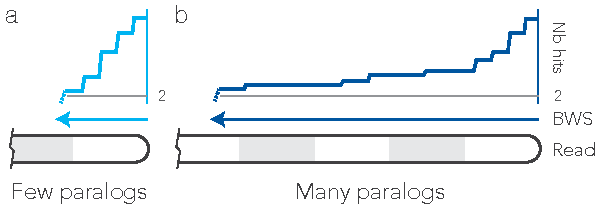
\includegraphics[scale=.84]{pushing_backward.pdf}
\end{center}
\caption{Estimating $N$ with the backward search. \textbf{(a)} The target
has no or few paralogs. It takes only a few iterations until the backward
search (BWS) finds fewer than 2 hits in the genome. \textbf{(b)} the
target has many paralogs. In this case it takes more iteration before the
query has fewer than 2 hits. The number of iterations above the threshold
is used as a statistic to estimate $N$.}
\label{fig_back}
\end{figure}

We can thus use the length of the largest query with 2 or more hits in the
genome as a statistic to estimate $N$ (see Materials and Methods).


\subsection{Super reads}
\label{sec_super}

As mentioned above, our strategy to map reads with high confidence is to
test whether the target is unique. Intuitively, a read that maps to a
sequence without paralog in the genome is very likely to be mapped to the
correct location.

We designed another estimation procedure based on the backward search,
where this time we use the best candidate location and not the read as a
query. The principle, sketched in Figure~\ref{fig_supertest}a, is to
perform the backward search on 20-mers and to test whether the genome
contains a single hit (the candidate location). The rationale is that the
total number of 20-mers is approximately $10^{12}$, so the chances of
spurious random hits are very low, even in the largest known genomes.

For a complete test, the proposed location of the read is segmented in
20-mers overlapping by 10 nucleotides, as shown in
Figure~\ref{fig_supertest}b. The sequence is considered unique if all the
extracted 20-mers have a single hit in the genome.

\begin{figure}[t]
\begin{center}
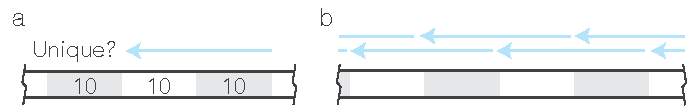
\includegraphics[scale=.75]{supertest.pdf}
\end{center}
\caption{Test for uniqueness. \textbf{(a)} Basic principle. After the
alignment stage, the sequence of the best hit is segmented in 20-mers. The
uniqueness of a given 20-mer is tested with the backward search.
\textbf{(b)} Complete test. The genomic location returned by the search
process is considered to be unique if all the 20-mers overlapping by 10
nucleotides are unique.}
\label{fig_supertest}
\end{figure}

While testing this procedure, we noticed that a class of reads were mapped
with higher confidence than ever reported before. The \emph{super reads},
as we called them, were those aligning perfectly to a unique location.

The extremely high mapping quality of super reads comes from an unexpected
property of the test depicted in Figure~\ref{fig_supertest}. To see why
they can be mapped with such confidence, consider a read aligning
perfectly with an incorrect sequence of the genome. Observe that for
this to happen, the read must contain an error that is perfectly
compensated in some duplicate of the target. This can only happen if $i.$
the target has a duplicate, $ii.$ the read contains an error, $iii.$ this
error matches the duplicate and $iv.$ the target and the duplicate are
otherwise identical.

\begin{figure*}[t]
\begin{center}
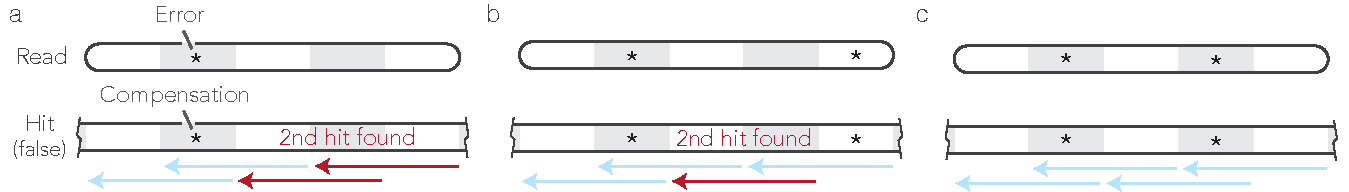
\includegraphics[scale=.79]{super_reads.pdf}
\end{center}
\caption{Properties of super reads. \textbf{(a)} Incorrect perfect
alignment. For a read to align perfectly to an incorrect sequence, the
read must contain an error (star in the read) and the incorrect nucleotide
must match a paralog (star in the hit). This is not a super read because
some extracted 20-mers are not unique (red arrows). \textbf{(b)} Incorrect
perfect alignment with several errors. Adding compensated errors is not
always sufficient to make 20-mers unique. To much space between errors can
leave 20-mers that are not unique, in which case the read is not super.
\textbf{(c)} Incorrectly mapped super reads. If the compensated errors are
in odd-numbered 10-mers (grey boxes), then all the extracted 20-mers are
unique and the read is super. Those conditions are exceedingly rare, so
super reads are mapped with high confidence.}
\label{fig_supread}
\end{figure*}

But those conditions are not sufficient to make a read \emph{super}. As
shown in Figure~\ref{fig_supread}a, the mapping location would not be
considered unique because there would exist at least one 20-mer where the
target and its dupliate are identical. For a read of size 50, the
duplicate can be overlooked only if there are at least two errors in the
read that match the paralog.

But as shown in Figure~\ref{fig_supread}b, this is still not sufficient
for a wrongly mapped read to qualify as \emph{super}. For this, every
second 10-mer must contain an error that is exactly compensatd in the
duplicate, as indicated in Figure~\ref{fig_supread}c. In this
configuration, the errors mask the presence of a duplicate on all the
tested 20-mers and the incorrect target location is considered unique.
There are other scenarios where a super read is mapped to an incorrect
location, but they involve even more compensated errors so they can be
neglected.


\subsection{MEM Mapper Prototype}

We implemented the mapping strategy presented in Figure~\ref{fig_tree} in
a prototype mapper called MEM Mapper Prototype (MMP). We used plain
mapping algorithms to better highlight the benefits of building a mapper
for faithfulness. The index consists of a standard FM-index of the genome
and its reverse complement~\citep[the implementation is detailed in
ref.][]{blog}. We also added an auxiliary lookup table storing the states
of the bacwkard search for all possible 12-mers, allowing us to skip the
first 12 iterations for every query. This lookup table has a fixed size of
256~MB. Sequence alignment is carried out using a version of the
Needleman-Wunsch algorithm~\cite{pmid5420325} with an option to abort if
the score of the current best hit is exceeded (continuing the algorithm is
useless to find the optimal location of the read). Mapping quality is
computed as detailed in the Materials and Methods section.

We set up a test using the genomes of \textit{Drosophila melanogaster}
(the fruit fly), \textit{homo sapiens} (modern humans) and \textit{Pinus
taeda} (a north American species of pine). The high-level features of the
genomes are summarized in Table~\ref{table_genomes}. We included
\textit{Drosophila} and human as model organisms with high-quality genome
assemblies, and pine as a non-model organism with a very complex genome
and a draft assembly.

To set a baseline for comparison we used BWA-MEM and Bowtie2. The purpose
of the benchmark is to test faithfulness as a viable mapping strategy, not
to run a comprehensive survey of each mapper on the data set. Each mapper
was thus used with its default parameters (but we still passed the
non-optional error rate to MMP).

\begin{figure*}[t]
\begin{center}
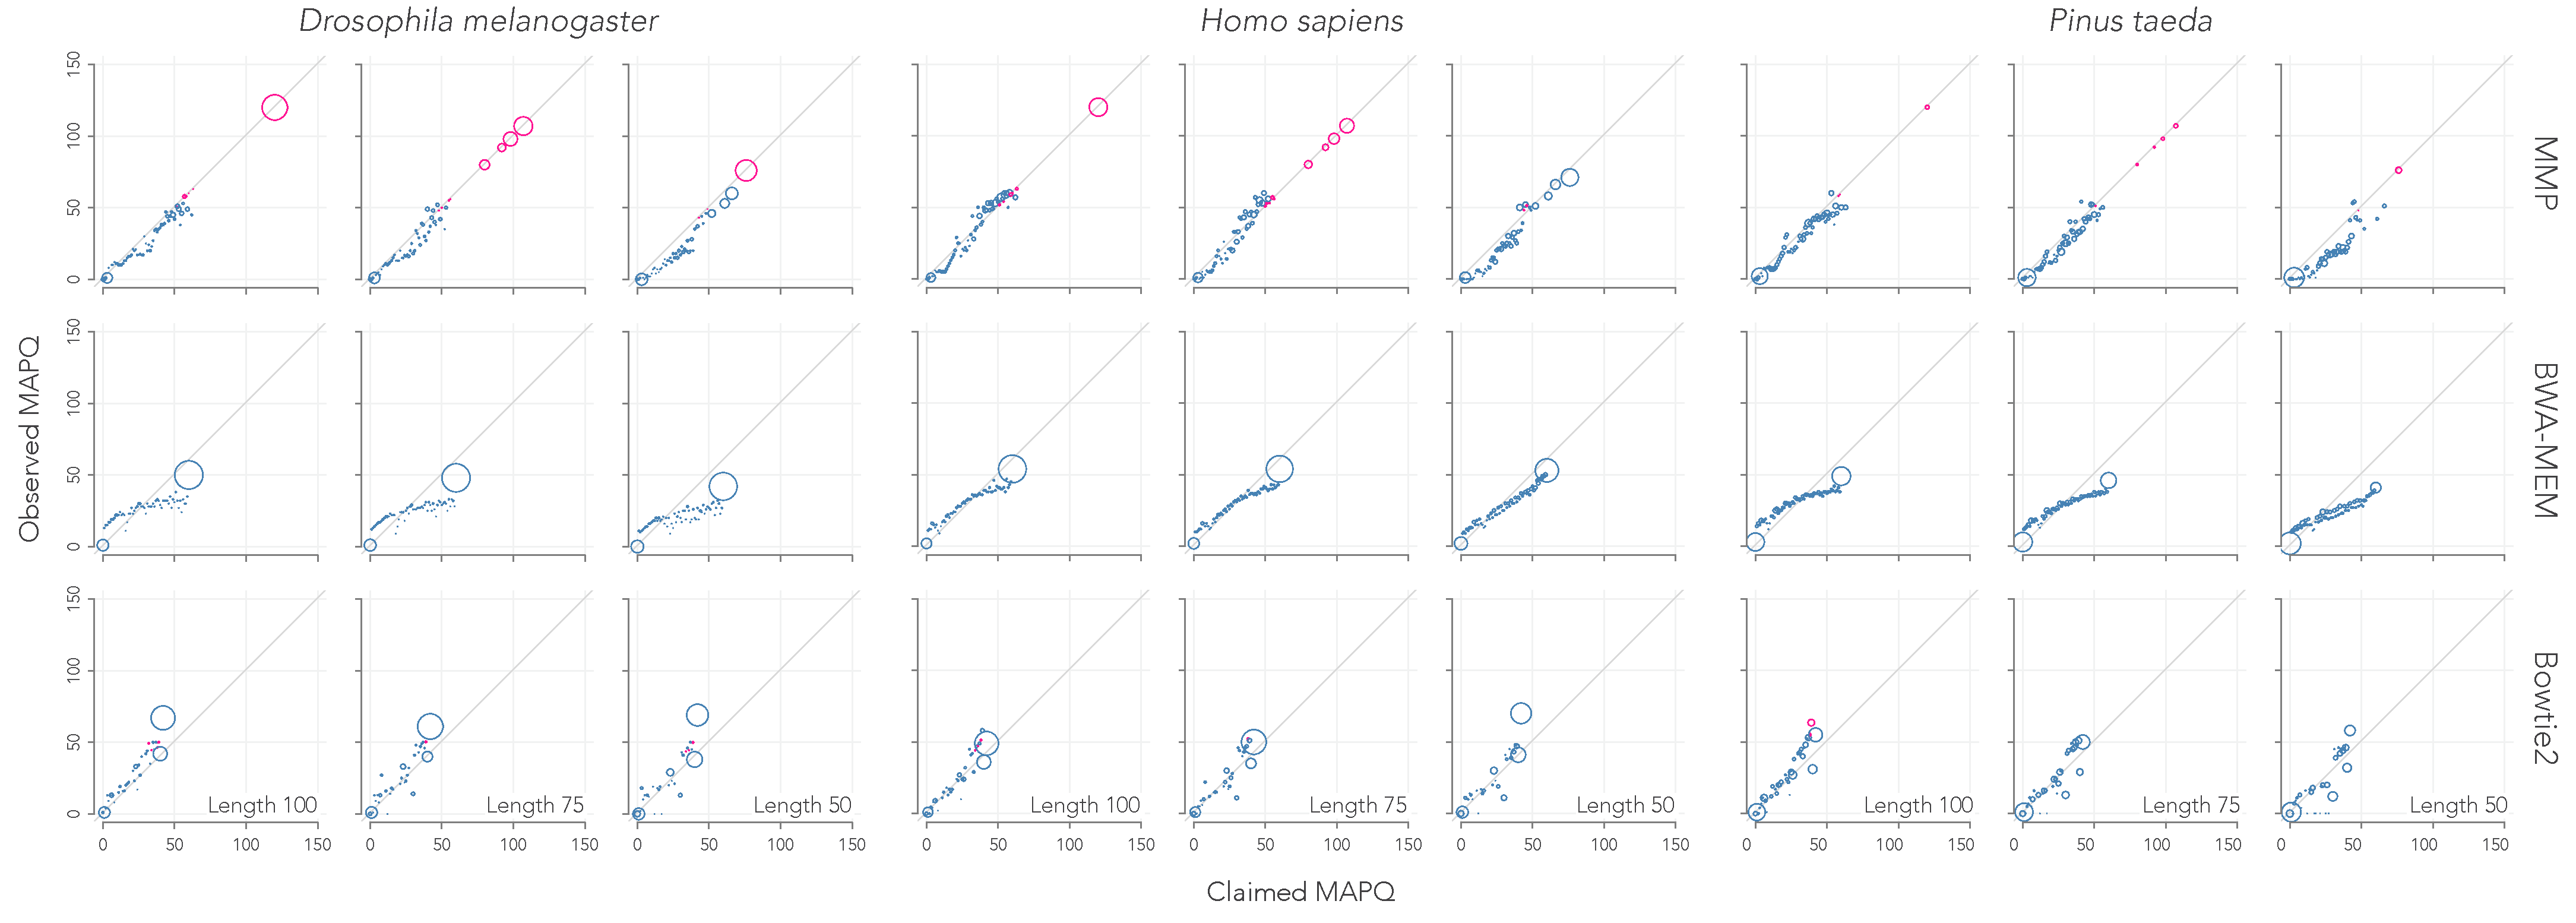
\includegraphics[scale=.24]{fig_faith.pdf}
\end{center}
\caption{Faithfulness with 1\% error rate. The observed mapping quality
(MAPQ) is plotted against the value computed by MMP, BWA-MEM or Bowtie2.
The data is showed for reads of size 100, 75 or 50, sampled from the
genome of the fruit fly (\textit{D. melanogaster}), of modern humans
(\textit{H. sapiens}) or of the pine (\textit{P. taeda}). The size of the
circle is proportional to the number of reads in the given category. Pink
circles indicate that no mapping error was observed, so that the observed
mapping quality was undefined. In this case one pseudo error was added if
the expected number of errors was higher than 1 (we should observe errors
but we did not), otherwise the observed mapping quality was set to the
claimed mapping quality (we should not observe errors and we did not).}
\label{fig_faith}
\end{figure*}

We measured faithfulness by comparing observed versus claimed MAPQ score
on simulated data. Figure~\ref{fig_faith} shows a series of scatter plots
at 1\% simulated error rate. The area of the circles is proportional to
the number of reads in the given category, and pink circles indicate that
the observed mapping quality had to be imputed because all the reads were
mapped correctly.

The faithfulness of MMP compares favorably to that of BWA-MEM and Bowtie2
because on average, the points lie closer to the diagonal. Importantly,
MMP explores a wider range of mapping qualities, allowing it to map reads
with extremely high confidence. Those high-confidence reads with MAPQ
above 60 are all super reads, and Figure~\ref{fig_faith} shows that in
typical mapping conditions, their number can be very high (up to two
thirds when mapping 100-mers in the \textit{Drosophila} genome).
Intuitively, the number of super reads goes down as the complexity of the
genome increases.

Similar analyses for reads with higher error rates are shown in
Supplementary Figure~\ref{fig_supp}. The faithfulness of MMP is equally
high at 2\% error rate, but it decreases substantially at 5\% and 10\%
error rates, showing that our strategy is valid only within the scope of
current short-read sequencing technologies.

\begin{figure}[t]
\begin{center}
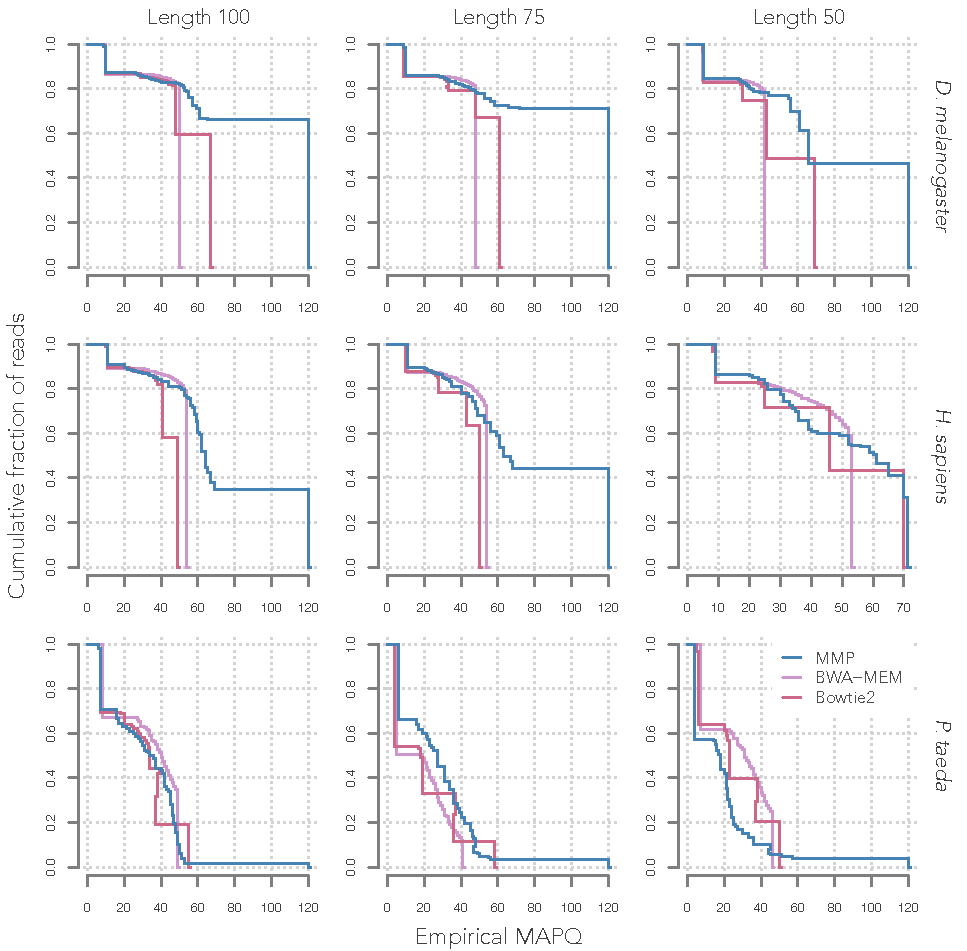
\includegraphics[scale=.54]{fig_acc.pdf}
\end{center}
\caption{Mapping accuracy with 1\% error rate. Plotted in each panel is
the cumulative fraction of the reads above a certain mapping quality for
MMP, BWA-MEM or Bowtie2. The score is computed empirically by sorting the
reads on MAPQ and computing the average mapping quality of the reads in
the top $x$\% for all values of $x$. The data is showed for reads of size
100, 75 or 50, sampled from the genome of the fruit fly (\textit{D.
melanogaster}), of modern humans (\textit{H. sapiens}) or of the pine
(\textit{P. taeda}).}
\label{fig_acc}
\end{figure}


Finally, it is important to evaluate the impact of faithfulness in terms
of accuracy, speed and memory footprint. Figure~\ref{fig_acc} shows that
the accuracy of MMP is competitive with that of BWA-MEM and Bowtie2
(recall that the mappers were used with default parameters). On the
\textit{Drosophila} genome, MMP is more accurate at most confidence
levels, whereas there are more variations on the human and the pine
genomes. The worst case for MMP is that of 50-mers mapped in the pine
genome, perhaps because a MEM-only seeding strategy is not competitive in
such cases. Since the goal was never to optimize accuracy, those results
show that faithfulness is compatible with accuracy.

\begin{figure}[t]
\begin{center}
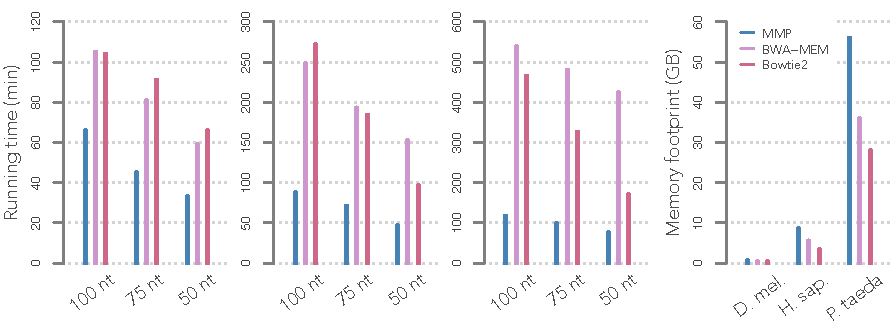
\includegraphics[scale=.58]{fig_timem.pdf}
\end{center}
\caption{Resource usage at 1\% error rate. \textbf{(a)} Speed. The running
time is plotted for MMP, BWA-MEM or Bowtie2. The data is showed for reads
of size 100, 75 or 50, sampled from the genome of the fruit fly
(\textit{D. melanogaster}), of modern humans (\textit{H. sapiens}) or of
the pine (\textit{P. taeda}). \textbf{(b)} Memory usage. The peak memory
footprint is plotted for the different mappers with reads from different
genomes (the memory footprint is the same for all read sizes).}
\label{fig_timem}
\end{figure}

In terms of speed, MMP is 2--4 faster than BWA-MEM and Bowtie2 on the
present data set (Figure~\ref{fig_timem}a), with a memory footprint that
is approximately 2--3 times higher (Figure~\ref{fig_timem}b). Part of the
speed up is due to the implementation and the larger stress on memory, but
the strategy highlighted in Figure~\ref{fig_tree} aims to reduce the
number of alignments when reads cannot be mapped accurately. For instance,
MMP spends 8.3\% of the time on incorrectly mapped reads, versus 29.2\%
and 12.5\% for BWA-MEM and Bowtie, respectively (100 nucleotide reads in
the human genome, data not shown).

Overall, Figures~\ref{fig_acc} and \ref{fig_timem} show that the
investment in faithfulness is paid back in several ways: First, it gives
access to very high confidence levels. Second, it auto-tunes accuracy by
better separating low from high-confidence reads. Third, it allows to save
time on low-confidence reads. Taken together, our results thus show that
faithful mapping is not only a viable strategy, it also opens
opportunities for further optimizations that can make the mapping process
more efficient.


\section{DISCUSSION}

Here we designed and implemented a strategy to map short reads faithfully.
The principles are based on key insight gained from models to compute
seeding probabilities~\cite{Filion619155}, showing that MEM seeds are
efficient only when the target has few paralogues (Figure~\ref{fig_MEM}).
This motivates the design of a strategy where we first estimate the copy
number of the target (Figure~\ref{fig_back}) to dispatch reads to
different mapping subroutines (Figure~\ref{fig_tree}). This amounts to
allocating more resources to the most mappable reads~\cite{pmid22276185}.
This process revealed the existence of super reads, \textit{i.e.}, reads
that can be mapped with extremely high confidence
(Figures~\ref{fig_supertest} and \ref{fig_supread}), together setting the
basis of an efficient mapping strategy. We wrote a mapper based on this
strategy and we showed that it is competitive with BWA-MEM and Bowtie
(Figures~\ref{fig_faith}, \ref{fig_acc} and \ref{fig_timem}). Importantly,
the mapping process itself relies only on standard algorithm, so all the
benefits of the mapper come from faithfulness. Overall, this demonstrates
that improving faithfulness is a fruitful strategy to improve short-read
mappers.


\subsection{Estimating MAPQ}

Our previous work indicated that seeding is the critical step to
estimating mapping quality~\cite{Filion619155}. Computing the seeding
probabilities requires to know the error rate of the sequencer, the number
$N$ of paralogs of the target and their sequence divergence. The error
rate may be known with reasonable accuracy, but $N$ is typically less
reliable, which is one of the major difficulties with the strategy
developed here and the main reason why the mapping quality of MMP is
sometimes inaccurate (Figure~\ref{fig_faith}).

\texttt{sesame} computes probabilities with high
precision~\cite{Filion619155}, but several practical considerations
obstruct the estimation of $N$. The first is that estimating $N$ must be
fast. The method depicted in Figure~\ref{fig_back} only requires a
backward search at each end of the read, but it provides only two
measurements and is thus inaccurate. The second practical consideration is
that the left and right halves of the read may have different $N$. This is
the case, for instance, when the read straddles a transposon, where the
end in the transposon may have a high copy number and the other end may be
unique. The final consideration is that the evolutionary model assumes
that the paralogs drift away from each other at the same speed, which
ignores their genealogy. The estimation thus provides a \emph{proxy}
estimate of $N$, as if the read behaved according to our assumptions.

When there is evidence that the target is unique, the mapping quality is
commensurate with the belief that $N = 0$. In this case, it would be more
appropriate to describe the estimation of $N$ as measuring the probability
that a paralog was missed during the search. This is the logic that
explains the high mapping quality of super reads: when there is a perfect
match, the screening process described in Figure~\ref{fig_supertest}
implicitly rules out many scenarios where the target has a paralog in the
genome (Figure~\ref{fig_supread}), so that only rare events remain
possible. The calculations are completely independent from \texttt{sesame}
and even of the seeding process, they are thus very general and can be
used in any mapper based on the FM-index without further modifications. In
this sense, the introduction of super reads constitutes one of the most
important contributions of the present work.

Figure~\ref{fig_faith} suggests that the mapping quality of super reads is
properly calibrated but the representation is somewhat self serving
because in reality the true error rate cannot be computed in this case. A
mapping quality of 120 means one error every 2000 sequencing runs
(assuming that all 500 million reads of each run are super reads), meaning
that in practice one will never observe a mapping error for reads in this
category. The exact MAPQ score above 120 does not matter, as long as all
the reads are mapped correctly. For super reads of size 50, the mapping
quality is around 75 and it seems to be correctly estimated based on the
simulated data from the human genome (sixth panel from the left in
Figure~\ref{fig_faith}), there is thus no reason to doubt the other
estimates.

Mapping quality increases with the read length (Figure~\ref{fig_faith}),
but longer reads are less likely to be super. The reason is simply that
they are more likely to contain a sequencing error. This appears on the
rightmost panel of Figure~\ref{fig_faith}, where in the pine genome, there
are more reads of size 50 that map without mistakes than reads of size
100. This suggests that the strategy of MMP could be improved by running
the uniqueness test of Figure~\ref{fig_supertest} only on the parts of the
reads that have a perfect match in the genome. This would allow more reads
to be labelled as super, though with a somewhat lower confidence. But
overall, future improvements are more likely to come from better indexing,
as we explain below.


\subsection{Performance}

Figure~\ref{fig_timem} shows that MMP is 2--4 times faster than BWA-MEM
and Bowtie2, while using 2--3 times more memory (trading speed for memory
in MMP was a design decision based on the standards of present-day
hardware). It is probable that BWA-MEM and Bowtie2 would also run 2--3
times faster with an equally large index size so the higher speed of MMP
cannot be interpreted as higher performance. It is otherwise important to
bear in mind that our benchmark is not entirely fair because BWA-MEM and
Bowtie2 are general mappers: they have to meet the demand on many
different tasks so they cannot use some of the shortcuts implemeted in
MMP.

Overall the mappers spend time on very different tasks: BWA-MEM and
Bowtie2 use sophisticated methods to refine the candidate set after
seeding, for instance by extending the set through re-seeding. In
comparison MMP either tests all the candidates (when $N \leq 20$) or tests
only one (when $N > 20$), but it never extends the candidate set. The
extra work that has to be carried out by MMP consists of estimating $N$
(Figure~\ref{fig_back}), testing uniqueness (Figure~\ref{fig_supertest})
and computing mapping qualities with \texttt{sesame}. The latter is
negligible, but the first two represent a significant part of the running
time (around 10--20\% with large variations on different data sets). The
point of MMP is to demonstrate that these steps can be carried out fast
enough for a mapper to remain competitive.

However, it is wasteful to test uniqueness for every read. Unique
sequences can be flagged at indexing time so that no additional
computations are required at mapping time. For instance, if it is known
with absolute certainty that a locus has no paralog, then mapping quality
is extremely high throughout the locus (remember that spurious random hits
are easy to detect as soon as the reads are longer than approximately 30
nucleotides). With this kind of information, super reads would be
unnecessary and even higher mapping quality could be achieved on large
parts of the genome. Likewise, the number of paralogs $N$ of each locus
could be stored to save computation time and to obtain more accurate
estimates of the mapping quality throughout the genome. It is presently
unclear how to compute $N$ for every locus and how to annotate a genome
accordingly, but when practical solutions exist, faithful mapping will
gain speed and robustness.

The case of accuracy is interesting (Figure~\ref{fig_acc}). For  the
genome of \textit{Drosophila}, which is relatively simple, the benefits of
MMP  are evident, while they are mitigated for the more complex human and
pine genomes. MMP tends to ``give up'' easily to save time on difficult
reads, so it may underperform when these cases are very frequent. One
straightfoward way to improve the accuracy would be to map the reads with
a more sensitive strategy when their mapping quality is too low. For
instance, using skip seeds like Bowtie2 may redeem such reads, if one is
willing to spend the time to give them a second chance. This would not be
a problem because the seeding probabilities of skip seeds are readily
available in \texttt{sesame}. The only downside would be a loss of speed,
but the mapper would still be faithful.


\subsection{Benefits of faithul mapping}

The idea of developing a faithful heuristic for better calibration was
originally proposed in BLAST~\cite{pmid2231712}. The speed gain over its
ancestor FASTP was very substantial, whereas this is not the case for MMP.
Modern short-read mappers are highly optimized so it is unlikely that a
10-fold speedup could be gained by just calibrating the heuristics they
rely on. That said, MMP demonstrates that there is room for improvement by
exploring new ways to efficiently estimate faithfulness.

The present work focuses on general mapping tasks in eukaryotic genomes,
but faithful read mappers may find much more interesting applications,
such as when the reference contains several variants of the same
sequences. This is the case for the genome of hybrid species or of
heterozygote individuals where each sequence has $N \geq 1$ duplicates in
the reference. In this case, the challenge is to estimate the confidence
that the read maps to one genome or the other. MMP could be used for this
kind of problem, but a more specialized method that capitalizes on the key
information $N \geq 1$ would be more appropriate. For instance, the time
spent looking for super reads is wasted in this context because they
cannot occur (not a single sequence is unique). A more specialized method
dedicated to calibrating low mapping quality is expected to give better
results.

Another case of interest is when the DNA sample is contaminated and needs
to be mapped to several species. This occurs when working with primates
because experimenters can contaminate the biological material with their
own DNA, or simply when the source of the DNA is unknown. In such cases,
only few sequences are expected to have no duplicate in the reference. In
particular, if the genomes of interest are relatively close, the copy
number will usually be equal to the number of genomes. In such cases, a
general faithful mapper such as MMP is expected to give decent results,
even though it was not tested in this context. More generally, we expect
faithful mapping algorithms to find other applications in many areas of
biology. 


\section{CONCLUSION}

Faithfulness is an important feature of the mapping process. We have
demonstrated that it is possible to achieve faithful mapping while
remaining competitive in terms of speed, accuracy and memory usage.
Exploring new algorithms for faithful mapping is a promising avenue of
research that can also bring benefits in speed and mapping quality.


\section{ACKNOWLEDGEMENTS}

We would like to thank Santiago Marco-Sola, Catalina Romero and Nicholas
Stroustrup for their critical comments on the manuscript.
This work was funded by the Spanish Ministry of Economy, Industry and
Competitiveness (MEIC, Plan Estatal PGC2018-099807-B-I00) and by the
European Research Council (Synergy Grant 609989). R.~C. was supported by
the People Programme (Marie Curie Actions) of the European Union's Seventh
Framework Programme (FP7/2007-2013) under REA grant agreement 608959. We
acknowledge the financial support of the MEIC to the EMBL partnership, the
Centro de Excelencia Severo Ochoa and the CERCA Programme / Generalitat de
Catalunya.




\subsubsection{Conflict of interest statement.} None declared.
\newpage

\bibliography{references,pubmed}
\bibliographystyle{nar}

%\begin{thebibliography}{4}
%
%% Format for article
%\bibitem{1}
%Author,A.B. and Author,C. (1992)
%Article title.
%\textit{Abbreviated Journal Name}, \textbf{5}, 300--330.
%
%% Format for book
%\bibitem{2}
%Author,D., Author,E.F. and Author,G. (1995)
%\textit{Book Title}.
%Publisher Name, Publisher Address.
%
%% Format for chapter in book
%\bibitem{3}
%Author,H. and Author,I. (2005)
%Chapter title.
%In
%Editor,A. and Editor,B. (eds),
%\textit{Book Title},
%Publisher Name, Publisher Address,
%pp.\ 60--80.
%
%% Another article
%\bibitem{4}
%Author,Y. and Author,Z. (2002)
%Article title.
%\textit{Abbreviated Journal Name}, \textbf{53}, 500--520.
%
%\end{thebibliography}

\end{document}
